\newpage
\section{Manuel utilisateur}
\label{sec:manuel}
\subsection{Prérequis}
Pour faire tourner CHESS, il faut :
\begin{itemize}
\item Java JDK 1.8 ou supérieur installé sur la machine ;
\item Eclipse IDE ;
\item La librairie \texttt{log4j-1.2.17.jar} fournie par l'enseignant.
\end{itemize}
\subsection{Importer et configurer le projet sous Eclipse}
\paragraph{Importer le projet :}
\begin{enumerate}
\item Ouvrir Eclipse
\item Aller dans \texttt{File} $\rightarrow$ \texttt{Import}
\item Choisir \texttt{Existing Projects into Workspace}
\item Sélectionner le dossier du projet et valider
\end{enumerate}
\paragraph{Ajouter la librairie Log4j :}
\begin{enumerate}
\item Clic droit sur le projet $\rightarrow$ \texttt{Properties}
\item Aller dans \texttt{Java Build Path} $\rightarrow$ \texttt{Libraries}
\item Cliquer sur \texttt{Add External JARs} et sélectionner \texttt{log4j-1.2.17.jar}
\item Valider avec \texttt{Apply and Close}
\end{enumerate}
\paragraph{Lancer le jeu :}
\begin{enumerate}
\item Aller dans le package \texttt{gui}
\item Faire un clic droit sur \texttt{MainGUI.java}
\item Choisir \texttt{Run As} $\rightarrow$ \texttt{Java Application}
\end{enumerate}
\subsection{Utilisation du jeu}
\paragraph{Page d'accueil} Au lancement, on arrive sur la page d'accueil avec deux boutons :
\begin{itemize}
\item \textbf{VS BOT} : jouer contre l'ordinateur. Un menu s'ouvre pour choisir la difficulté (Facile, Moyen ou Difficile) ;
\item \textbf{VS HUMAIN} : jouer à deux joueurs sur la même machine, chacun son tour.
\end{itemize}
\begin{figure}[H]
\centering
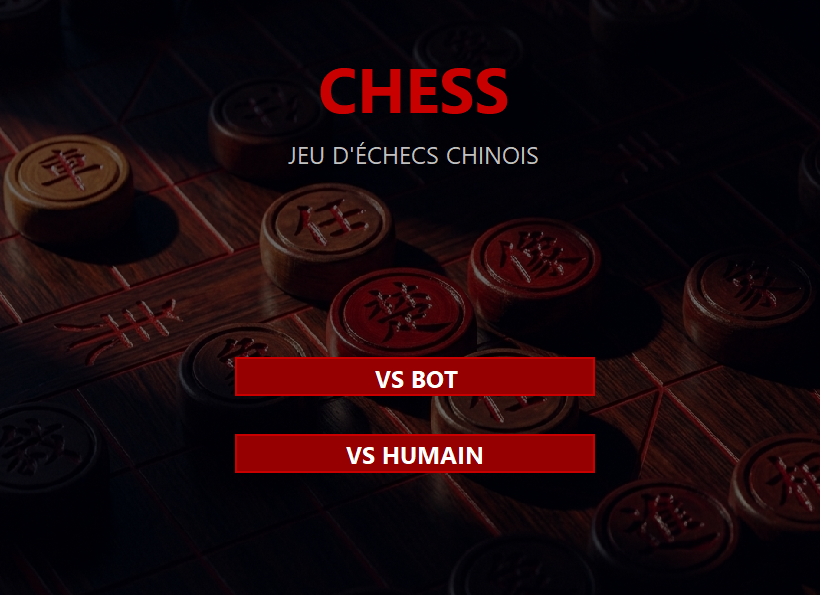
\includegraphics[width=10cm, height=7cm]{images/acceuil.png}
\caption{Page d'accueil de CHESS}
\label{fig:accueil}
\end{figure}
\paragraph{Pendant une partie}
\begin{itemize}
\item Pour jouer, on clique d'abord sur une de nos pièces — les cases où elle peut aller s'affichent en surbrillance ;
\item On clique ensuite sur une case en surbrillance pour effectuer le déplacement ;
\item Si on clique ailleurs, la sélection est annulée ;
\item Les pièces capturées apparaissent dans les panneaux en haut (noires capturées) et en bas (rouges capturées) du plateau ;
\item L'historique des coups joués s'affiche dans le panneau à droite avec la couleur du joueur correspondant ;
\item L'indicateur en bas à droite montre en permanence à qui c'est le tour (RED ou BLACK).
\end{itemize}
\begin{figure}[H]
\centering
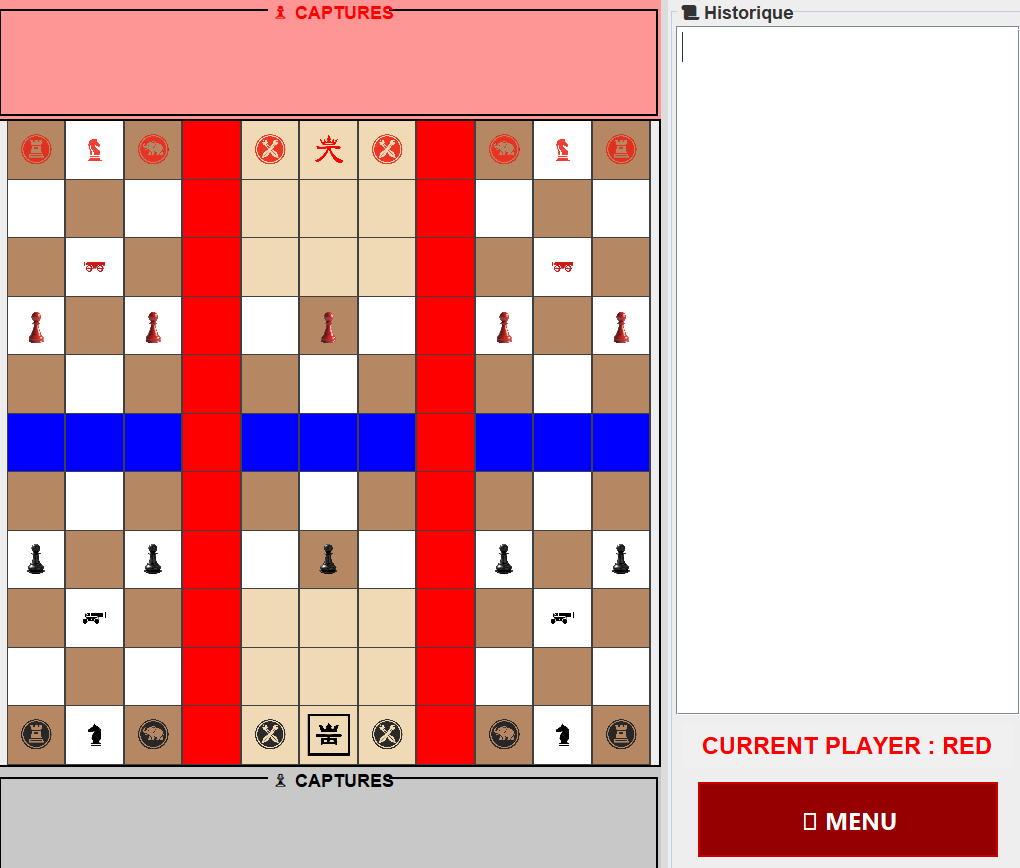
\includegraphics[width=13cm, height=9cm]{images/plateau.png}
\caption{Plateau de jeu pendant une partie}
\label{fig:partie}
\end{figure}
\paragraph{Menu en cours de partie} Le bouton \textbf{MENU} ouvre un dialogue avec trois options :
\begin{itemize}
\item \textbf{Reprendre} : ferme le menu et continue la partie ;
\item \textbf{Nouvelle Partie} : remet le plateau à zéro ;
\item \textbf{Quitter} : retourne à la page d'accueil.
\end{itemize}
\begin{figure}[H]
\centering
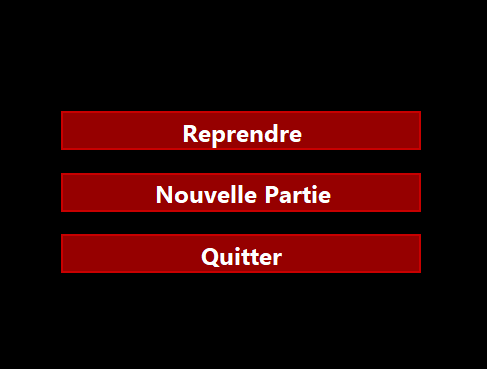
\includegraphics[width=6cm, height=5cm]{images/menu.png}
\caption{Menu en cours de partie}
\label{fig:menu}
\end{figure}
\paragraph{Fin de partie} Quand un joueur est en échec, une boîte de dialogue l'avertit. Quand il est en échec et mat, la partie se termine automatiquement et on ne peut plus jouer. 
